%%%%%%%%%%%%%%%%%%%%%%%%%%%%%%%%%%%%%%%%%%%%%%%%%%%
%% P3: Phenomenology of Particle Physics                         
%%
%% Author:  André Rubbia                   		 
%%
%% Figure 11.2 Angular dependence of the Mott scattering cross-section compared to the Rutherford formula.
%%
%% This work is licensed under the Creative Commons Attribution 4.0 International License. 
%% To view a copy of this license, visit http://creativecommons.org/licenses/by/4.0/ or 
%% send a letter to Creative Commons, PO Box 1866, Mountain View, CA 94042, USA.
%%
%%%%%%%%%%%%%%%%%%%%%%%%%%%%%%%%%%%%%%%%%%%%%%%%%%%

\documentclass[a4paper,10pt]{article}

\usepackage[T1]{fontenc}
\usepackage[utf8]{inputenc}
\usepackage{lmodern}
\usepackage[labelfont=bf]{caption}
\usepackage{upgreek}

\usepackage{tikz}
\usepackage{pgfplots}
\pgfplotsset{compat=1.17}
\usepgfplotslibrary{ternary}
\usepgfplotslibrary{fillbetween}
\usepgfplotslibrary{external}

\def\d{\mathrm{d}}

\begin{document}

%%%%%%%%%%%%%%%   FIGURE  %%%%%%%%%%%%%%%%%%%%%%%%%%%%%%
\begin{figure}[htb]
\begin{center}
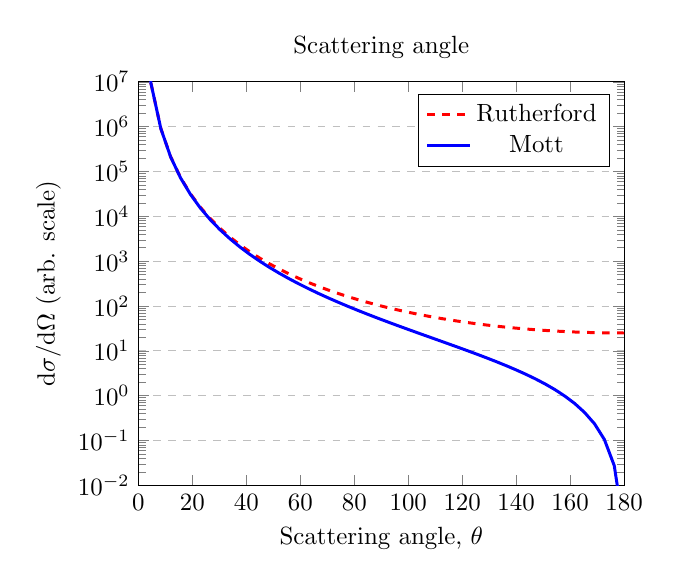
\begin{tikzpicture}[scale=0.9]
\begin{semilogyaxis}[
    title={Scattering angle},
    xlabel={Scattering angle, $\theta$},
    ylabel={${\d \sigma}/{\d\Omega}$ (arb. scale)},
    xmin=0, xmax=180,
    ymin=0.01, ymax=1e7,
    xtick={0,20,40,60,80,100,120,140,160,180},
    ytick={1e-2,1e-1,1e0,1e1,1e2,1e3,1e4,1e5,1e6,1e7},
    legend pos=north east,
    ymajorgrids=true,
    grid style=dashed,
]
\addplot[domain=1:180,samples=50,
    color=red,very thick, dashed]
    {0.25e2/sin(x/2)^4};
\addplot[domain=1:180,samples=50,
    color=blue,very thick]
    {0.25e2/sin(x/2)^4*(1-sin(x/2)^2};
     \legend{Rutherford, Mott}
\end{semilogyaxis}
\end{tikzpicture}
%
\hspace{0.2cm}
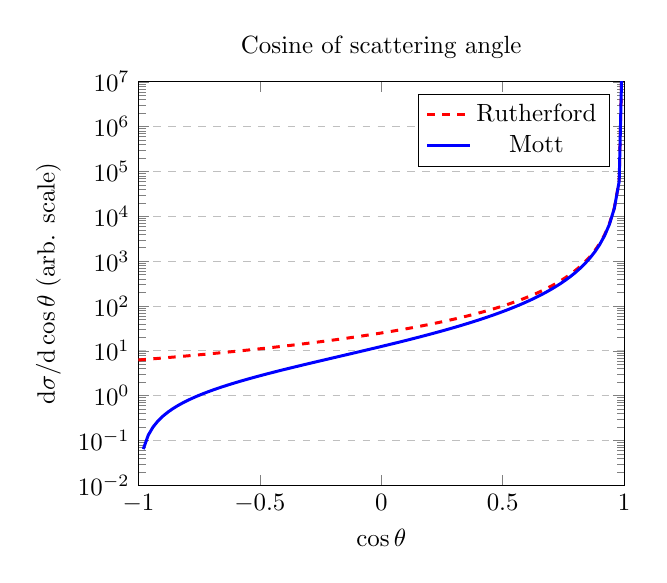
\begin{tikzpicture}[scale=0.9]
\begin{semilogyaxis}[
    title={Cosine of scattering angle},
    xlabel={$\cos\theta$},
    ylabel={${\d \sigma}/{\d \cos\theta}$ (arb. scale)},
    xmin=-1, xmax=1,
    ymin=0.01, ymax=1e7,
    xtick={-1,-0.5,-0,0.5,1},
    ytick={1e-2,1e-1,1e0,1e1,1e2,1e3,1e4,1e5,1e6,1e7},
    legend pos=north east,
    ymajorgrids=true,
    grid style=dashed,
]
\addplot[domain=-1:1,samples=100,
    color=red,very thick, dashed]
    {0.25e2/(1-x)^2};
\addplot[domain=-1:1,samples=100,
    color=blue,very thick]
    {0.25e2*0.5*(1+x)/(1-x)^2};
     \legend{Rutherford, Mott}
\end{semilogyaxis}
\end{tikzpicture}
\caption{Angular dependence of the Mott scattering cross-section
compared to the Rutherford formula: (left) as a function
of the scattering angle $\theta$; (right) as a function of $\cos\theta$.}
\end{center}
\end{figure}
%%%%%%%%%%%%%%%   FIGURE  %%%%%%%%%%%%%%%%%%%%%%%%%%%%%%
%

\end{document}
